%
% beugung-herleitung.tex -- Herleitung aus WsComm2-Vorlesung
%
%
% !TEX root = ../../buch.tex
% !TEX encoding = UTF-8
%

\section{Anwendungsbeispiel: Beugung elektromagnetischer Wellen}
\kopfrechts{Anwendungsbeispiel: Beugung elektromagnetischer Wellen}

In der drahtlosen Kommunikation werden die Fresnel-Integrale für 
\index{drahtlose Kommunikation}%
die Beugung von Signalen an einer sogenannten Schneide gebraucht.
\index{Schneide}%
Diese Schneide ragt als Hindernis in die direkte 
Linie zwischen Sender und Empfänger
\index{Sender}%
\index{Empfanger@Empfänger}%
und sorgt damit für Verluste auf dem Sendeweg.
\index{Verlust}%
In den folgenden Abschnitten wird schrittweise an
die Formel für diese Verluste herangegangen,
zuerst mit einer einseitigen und anschliessend
mit der zweiseitigen Berechnung.

\subsection{Einseitige Verlustberechnung}
%
% fig-einseitig.tex
%
% (c) 2026 Prof Dr Andreas Müller
%
\begin{figure}
\centering
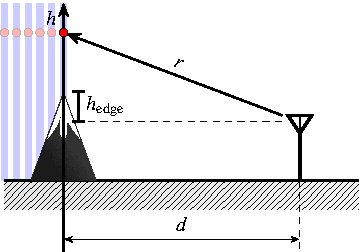
\includegraphics{papers/fresnel/images/einseitig.pdf}
\caption{Darstellung der einseitigen Verlustberechnung an einer Schneide,
Wellenfront eintreffend von links.
\label{fresnel:Diff-loss-einseitig-abb}}
\end{figure}


\subsubsection{Beschreibung der Geometrie}\label{fresnel:Beispiel-Geometriebeschrieb}
Als Ausgangspunkt für die einseitige Verlustberechnung wird die Geometrie wie in 
Abbildung~\ref{fresnel:Diff-loss-einseitig-abb} definiert:
\begin{itemize}
    \item
    Auf der rechten Seite steht eine Antenne als Empfänger.
\index{Antenne}%
    \item
    Auf der linken Seite steht ein Hindernis, eine sogenannte Schneide.
    \item 
    $d$ sei der horizontale Abstand vom Empfänger zur Schneide.
    \item 
    $h$ sei die Höhe des Ausgangspunktes einer Kugelwelle direkt über der Schneide.
    \item
    $h_{\text{edge}}$ sei die Höhe, welche die Schneide in die direkte Linie zwischen Sender und Empfänger hineinragt.
    \item 
    $r$ sei die Distanz vom Empfänger zum Ausgangspunkt einer Kugelwelle.
\index{Kugelwelle}%
\end{itemize}
Die Distanz $r$ ergibt sich über die Pythagoras-Formel als
\index{Pythagoras}%
\[
r(h) 
= 
\sqrt{d^2 + h^2}
=
d \sqrt{1 + \frac{h^2}{d^2}}.
\]
Da in den meisten Fällen die Distanz $d$
um ein Vielfaches grösser ist als die Höhe $h$,
kann mit der Taylor-Approximation der Wurzelfunktion die Distanz vereinfacht werden zu
\index{Taylor-Approximation}%
\begin{equation}
    r(h)
    =
    d \sqrt{1 + \frac{h^2}{d^2}}
    \approx
    d \biggl( 1 + \frac{h^2}{2d^2} \biggr)
    =
    d + \frac{h^2}{2d}.
    \label{fresnel:Distanz-R-Taylor-einseitig}
\end{equation}


\subsubsection{Beschreibung der Ausgangswelle}
Die Antenne empfängt ein Signal von der linken Seite 
hinter der Schneide.
Bei kurzen Distanzen mag dieses Signal
wie eine Kreiswelle ausgehend von der Antenne aussehen.
Für längere Distanzen sieht sie aber nach dem huygensschen Prinzip \cite{fresnel:huygenssches-prinzip}
\index{huygenssches Prinzip}%
\index{Prinzip von Huygens}%
aus wie eine ebene Welle wie in Abbildung~\ref{fresnel:Diff-loss-einseitig-abb},
welche aus Kugelwellen mit Ausgangspunkten in verschiedenen Höhen besteht.

\subsubsection{Kugelwellen} % c und d aus Mail zusammenehmen
Diese Kugelwellen haben eine Amplitude $\psi$,
welche mit wachsender Distanz abnimmt.
Die gemessene Amplitude $\psi$ nach einer Distanz $r$ und einer Zeit $t$ kann mit
\begin{equation}
    \psi (r,t)
    =
    \psi_0 \cdot \frac{e^{j(\omega t -kr)}}{r}
\end{equation}
und den Definitionen
\begin{itemize}
    \item 
    $\psi_0$ als ursprüngliche Amplitude,
    \item 
    $\omega$ als Phasenverschiebung,
\index{Phasenverschiebung}%
    \item 
    $k = \frac{2 \pi}{\lambda}$ als Wellenzahl abhängig von $\lambda$ und
\index{Wellenzahl}%
    \item 
    $\lambda$ als spezifische Wellenlänge (z.\,B. rotes Licht mit $\qty{740}{\nano\metre}$)
\end{itemize}
berechnet werden.
Damit lässt sich nun jede Amplitude 
der Kugelwellen oberhalb der Schneide berechnen,
indem für $r$ die entsprechende 
Distanz aus der Gleichung~\eqref{fresnel:Distanz-R-Taylor-einseitig} eingesetzt wird:
\begin{equation}
    \psi(r,t)
    =
    \psi_0 \cdot \frac{\exp\left(j(\omega t -kr)\right)}{r}
    \approx
    \psi_0 \cdot \frac{\exp\biggl(j\omega t -jk\biggl(d+\displaystyle\frac{h^2}{2d}\biggr)\biggr)}{d}.
    \label{fresnel:Amplitude-r-komplett-einseitig}
\end{equation}

\subsubsection{Approximation}
Die Verlustberechnung dient als Approximation.
$h$ ist im Vergleich zu $d$ sehr klein,
weshalb $r$ nur wenig ändert,
wenn sich $h$ ändert.
Die Signalwege sind folglich ungefähr gleich lang, 
weshalb Abschwächungen als Faktor $1/d$ und Verzögerungen als Faktor $\omega t$ der Signale 
vernachlässigt werden können.
Die Gleichung~\eqref{fresnel:Amplitude-r-komplett-einseitig}
wird somit zu
\begin{equation}
    \psi(r)
    =
    \psi_0 \cdot \exp\left(-jkr\right)
    \approx
    \psi_0 \cdot \exp\biggl(-jk\biggl(d+\frac{h^2}{2d}\biggr)\biggr).
    \label{fresnel:Amplitude-r-vereinfacht-einseitig}
\end{equation}

\subsubsection{Von der Wellenfront zur Wellendichte}
Für die weiteren Schritte ist es von Vorteil,
die Amplitude abhängig von $h$ zu diskretisieren.
Am einfachsten geht dies als Produkt von der Wellendichte
$\rho_{\psi}$ und diskreter Höhenabschnitte:
\begin{equation}
    % \psi
    % =
    % \rho_{\psi}\Delta h,
    % \qquad
    \psi(r)
    =
    \psi_0 \cdot e^{-jkr}
    =
    \rho_{\psi_0}\Delta h \cdot e^{-jkr}
    =
    \rho_{\psi }\Delta h,
    \qquad
    \rho_{\psi}
    =
    \frac{d\psi}{dh}.
    \label{fresnel:Wellendichte-umgestellt}
\end{equation}

\subsubsection{Überlagerung der Kugelwellen} % Superposition
Wir haben nun alle Werkzeuge, 
um die Kugelwellen mit Überlagerung
in ein einziges Signal $\psi_{\text{rx}}$ zusammenzufassen.
Zuerst wird die Gleichung~\eqref{fresnel:Amplitude-r-vereinfacht-einseitig}
über alle Höhen summiert:
\begin{subequations}
\label{fresnel:Kugelwellen-wellendichte-summiert}
    \begin{align}
        \psi_{\text{rx}}
        &=
        \sum_i \psi_0 \cdot e^{-jkr_i}
        =
        \psi_0 \cdot \sum_i \exp\biggl(-jk\biggl(d+\frac{h^2_i}{2d}\biggr)\biggr)\\
        &=
        \underbrace{\psi_0 \cdot e^{-jkd}}_{\displaystyle=\psi}
	\sum_i \exp\biggl(-jk\biggl(\frac{h^2_i}{2d}\biggr)\biggr).
    \end{align}
\end{subequations}
Anschliessend wird die Wellendichte von der Gleichung~\eqref{fresnel:Wellendichte-umgestellt}
eingesetzt:
\begin{equation}
    \psi_{\text{rx}}
    =
    \psi \cdot \sum_i \exp\biggl(-jk\biggl(\frac{h^2_i}{2d}\biggr)\biggr)
    =
    \rho_{\psi} \cdot \sum_i \exp\biggl(-jk\biggl(\frac{h^2_i}{2d}\biggr)\biggr) \Delta h.
    \label{fresnel:Kugelwellen-wellendichte-superpos}
\end{equation}

\subsubsection{Der Weg zu den Fresnel-Integralen}
Im Grenzwert $\Delta h\to 0$ wird die Summe in 
\eqref{fresnel:Kugelwellen-wellendichte-superpos}
%Die Gleichung~\eqref{fresnel:Kugelwellen-wellendichte-superpos}
%führt durch infinitesmal kleine Schritte
zum Integral
\begin{equation}
    \psi_{\text{rx}}
    =
    \rho_{\psi} \int_{h_{\text{edge}}}^{\infty} \exp\biggl(-jk\biggl(\frac{h^2}{2d}\biggr)\biggr) \,dh
    =
    \rho_{\psi} \int_{h_{\text{edge}}}^{\infty} \biggl(\cos \frac{kh^2}{2d} - j \sin \frac{kh^2}{2d}\biggr) \,dh.
    \label{fresnel:Kugelwellen-wellendichte-integral}
\end{equation}
Durch Zerlegung und Grenztausch in zwei Integrale mit Beginn bei 0
erhalten wir
\begin{equation}
    \psi_{\text{rx}}
    =
    \underbrace{\rho_{\psi} \int_{0}^{\infty} \biggl(\cos \frac{kh^2}{2d} - j \sin \frac{kh^2}{2d}\biggr) \,dh}_{\text{Gesamte Signalstärke}}
    -
    \underbrace{\rho_{\psi} \int_{0}^{h_{\text{edge}}} \biggl(\cos \frac{kh^2}{2d} - j \sin \frac{kh^2}{2d}\biggr) \,dh,}_{\text{Verlorene Signalstärke durch Schneidenbeugung}}
    \label{fresnel:Beispiel-Integral-ohne-fresnel}
\end{equation}
welche gewisse Ähnlichkeiten mit den 
Fresnel-Integralen~\eqref{fresnel:integral-C-S} aufweisen.
Mit der Substitution% von $t$ mit $h$ wird die Gleichung zu
\[
t(h)
=
h\sqrt{\frac{k}{\pi d}}
\quad
\Rightarrow
\quad
\frac{dh}{dt}
=
\sqrt{\frac{\pi d}{k}}
\quad
\Rightarrow
\quad
dh
=
\sqrt{\frac{\pi d}{k}} \,dt
\]
können die Integrale in
\eqref{fresnel:Kugelwellen-wellendichte-superpos}
%und kann
nach $C$
\begin{equation*}
    \int_{0}^{h_{\text{edge}}} \cos \biggl(\frac{k}{2d}h^2\biggr) \,dh
    =
    \sqrt{\frac{\pi d}{k}} \int_{0}^{h_{\text{edge}}\sqrt{\frac{k}{\pi d}}} \cos \biggl(\frac{\pi}{2}t^2\biggr) \,dt
    =
    \sqrt{\frac{\pi d}{k}} C(v)
\end{equation*}
und ebenso nach $S$
\begin{equation*}
    \int_{0}^{h_{\text{edge}}} \sin \biggl(\frac{k}{2d}h^2\biggr) \,dh
    =
    \sqrt{\frac{\pi d}{k}} \int_{0}^{h_{\text{edge}}\sqrt{\frac{k}{\pi d}}} \sin \biggl(\frac{\pi}{2}t^2\biggr) \,dt
    =
    \sqrt{\frac{\pi d}{k}} S(v)
\end{equation*}
umgestellt werden.
Das ganze Integral~\eqref{fresnel:Beispiel-Integral-ohne-fresnel}
ergibt sich dann zu
\begin{equation}
    \psi_{\text{rx}} (v)
    =
    \rho_{\psi} \sqrt{\frac{\pi d}{k}} \cdot \biggl[\frac{1}{2} - C(v) -j\biggl(\frac{1}{2}-S(v)\biggr)\biggr]
    \label{fresnel:Beispiel-Fresnelgleichung-einseitig}
\end{equation}
mit dem sogenannten \emph{Fresnel-Parameter}
\index{Fresnel-Parameter}%
\begin{equation}
    v
    =
    h_{\text{edge}} \sqrt{\frac{k}{\pi d}}
    \quad
    \overset{k = \frac{2 \pi}{\lambda}}{=}
    \quad
    h_{\text{edge}} \sqrt{\frac{2}{\lambda d}}.
    \label{fresnel:Fresnel-Parameter-einseitig}
\end{equation}

\subsubsection{Schlussfolgerung}
% \subsubsection{Intermezzo: $\unit{\decibel}$-Berechnungen}
Mit der erhaltenen Formel aus der Gleichung~\eqref{fresnel:Beispiel-Fresnelgleichung-einseitig}
und dem Fresnel-Parameter~\eqref{fresnel:Fresnel-Parameter-einseitig}
lässt sich nun der Verlust berechnen.
\index{Verlust}%
Als kleiner Einschub sei hier angemerkt,
dass in der Elektrotechnik keine Verhältnisse
\index{Elektrotechnik}%
zwischen Amplituden berechnet werden,
nur zwischen Leistungen.
Meist wird dies gelöst,
indem der absolute Wert der Amplitude quadriert wird,
also z.\,B. $|\psi_{\text{rx}} (v)|^2$.
Damit lässt sich der Verlust $L$ schreiben als
\begin{equation}
    L(v)
    =
    \frac{|\psi_{\text{gesendet}}|^2}{|\psi_{\text{verloren}}|^2}
    \approx
    \frac{|\psi_{\text{rx}} (-\infty)|^2}{|\psi_{\text{rx}} (v)|^2}
    =
%    \dots
%    =
    \frac{2}{\left|\frac{1}{2}-C(v)\right|^2 + \left|\frac{1}{2}-S(v)\right|^2}.
    \label{fresnel:Beispiel-diff-loss-einseitig}
\end{equation}
Für handlichere Werte und damit besserer Vergleichbarkeit
werden zusätzlich für die drahtlose Kommunikation Verluste in $\unit{\decibel}$
\index{dB}%
geschrieben, sprich es wird der Zehner-Logarithmus angewendet:
\[
L_{\unit{\decibel}} (v)
=
10 \cdot \log_{10} \frac{|\psi_{\text{rx}} (-\infty)|^2}{|\psi_{\text{rx}} (v)|^2}.
\]
Eine Halbierung der Sendeleistung würde also einem Verlust von
rund $\qty{3}{\decibel}$ entsprechen.

\subsection{Zweiseitige Verlustberechnung}
Bis jetzt wurden nur Verluste zwischen Schneide und Empfänger berechnet.
Es macht die Rechnungen zwar etwas einfacher, in den meisten Fällen
ist aber der Verlust zwischen Sender und Empfänger interessant.
%
% fig-beidseitig.tex
%
% (c) 2026 Prof Dr Andreas Müller
%
\begin{figure}
\centering
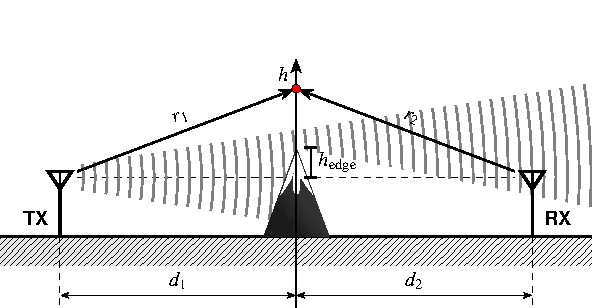
\includegraphics{papers/fresnel/images/zweiseitig.pdf}
\caption{Darstellung der Schneidenbeugung zwischen Sender und Empfänger.
\label{fresnel:knife-edge-abb}}
\end{figure}


\subsubsection{Unterschiede zur einseitigen Berechnung}
Die Abbildung~\ref{fresnel:knife-edge-abb} zeigt den neuen Sachverhalt.
Es ist zwar keine ebene Welle mehr, welche auf die Schneide trifft,
dies hat aber nur eine Phasenverschiebung zur Folge,
welche aufgrund der grösseren Distanz entsteht.
Zusätzlich setzt sich die Weglänge $r$
nun aus den beiden Teilen $r_1$ und $r_2$ zusammen.

\subsubsection{Umstellung der neuen Distanz}
Die neue Distanz $r$ berechnet sich aus
\[
r
=
r_1 + r_2
\quad
\text{mit}
\quad
r_n
=
\sqrt{d_n^2 + h^2}
=
d_n \sqrt{1 + \frac{h^2}{d_n^2}}
\text{ für }
n = {1,2}.
\]
Da wie am Anfang von Abschnitt~\ref{fresnel:Beispiel-Geometriebeschrieb} definiert
die Distanzen bedeutend grösser sind als die Höhe der Schneide,
kann mit der Taylor-Approximation der Wurzelfunktion der Term von $r_n $ zu
\[
r_n
=
d_n \sqrt{1 + \frac{h^2}{d_n^2}}
\approx
d_n + \frac{h^2}{2d_n}
\]
vereinfacht werden und ergibt für die gesamte Distanz $r$ 
\begin{equation*}
    r
    \approx
    d_1 + d_2 + \frac{h^2}{2}\biggl(\frac{1}{d_1} + \frac{1}{d_2}\biggr)
    =
    d_1 + d_2 + h^2\biggl(\frac{d_1 + d_2}{2d_1d_2}\biggr).
\end{equation*}
Setzt man die neue Distanz $r$ in die Gleichung~\eqref{fresnel:Kugelwellen-wellendichte-summiert} ein, folgt
\begin{align}
        \psi_{\text{rx}}
        &=
        \psi_0 \cdot \sum_i \exp\biggl(-jk\biggl(d_1 + d_2 + h^2_i\frac{d_1 + d_2}{2d_1d_2}\biggr)\biggr)
\notag
\\
        &=
        \underbrace{\psi_0 \cdot e^{-jk(d_1 + d_2)}}_{\displaystyle =\psi}
	\sum_i \exp\biggl(-jk\biggl(h^2_i\frac{d_1 + d_2}{2d_1d_2}\biggr)\biggr).
\label{fresnel:Kugelwellen-wellendichte-summiert-beidseitig}
\end{align}
Unter genauer Betrachtung fällt auf,
dass die neue Gleichung~\eqref{fresnel:Kugelwellen-wellendichte-summiert-beidseitig} 
der vorherigen stark gleicht.
Im Grunde ändert sich lediglich der Parameter
\[
\frac{1}{d}
\quad
\text{zu}
\quad
\frac{d_1 + d_2}{d_1d_2},
\]
%welches
diese Modifikation kann
folglich auf den Fresnel-Parameter~\eqref{fresnel:Fresnel-Parameter-einseitig}
angewendet werden und ergibt den modifizierten Fresnel-Parameter
\begin{equation}
    v
    =
    h_{\text{edge}} \sqrt{2\frac{d_1 + d_2}{\lambda d_1 d_2}}.
    \label{fresnel:Fresnel-Parameter-beidseitig}
\end{equation}
%angewendet werden kann.% Parameter bleibt, wenn einer der Stationen viel weiter vom Knife-Edge weg ist, als der andere

\subsubsection{Schlussfolgerung}
Die Verluste lassen sich also mit derselben Formel
und einem modifizierten Fresnel-Parameter
\eqref{fresnel:Fresnel-Parameter-beidseitig}
berechnen.
Diese können entweder über die Abbildung~\ref{fresnel:Fresnel-Diagram}
ausgelesen oder mit den Formeln
%\begin{subequations}
    \begin{align*}
        v > 1: \quad
        -L_{\unit{\decibel}}
        &=
        20 \log_{10}v + \qty{13}{\decibel}
        \\
        v > -0.7: \quad
        -L_{\unit{\decibel}}
        &=
        20 \log_{10}\left(\sqrt{(v-0.1)^2 + 1} + v -0.1\right) + \qty{6.9}{\decibel}
        \\
        \text{sonst:} \quad
        -L_{\unit{\decibel}}
        &=
        10 \log_{10} L(v)
    \end{align*}
%\end{subequations}
angenähert werden. 
Ein interessanter
%Punkt zur Erwähnung
Spezialfall
ist $v=0$.
Die Spitze der Schneide befindet sich hier perfekt auf der Höhe der Sichtlinie von Sender und Empfänger.
Aus der Abbildung lässt sich ungefähr $\qty{6}{\decibel}$ auslesen,
was einem Verlust von $3/4$ der ursprünglichen Sendeleistung entspricht.

%
% fig-verluste.tex
%
% (c) 2026 Prof Dr Andreas Müller
%
\begin{figure}
    \centering
    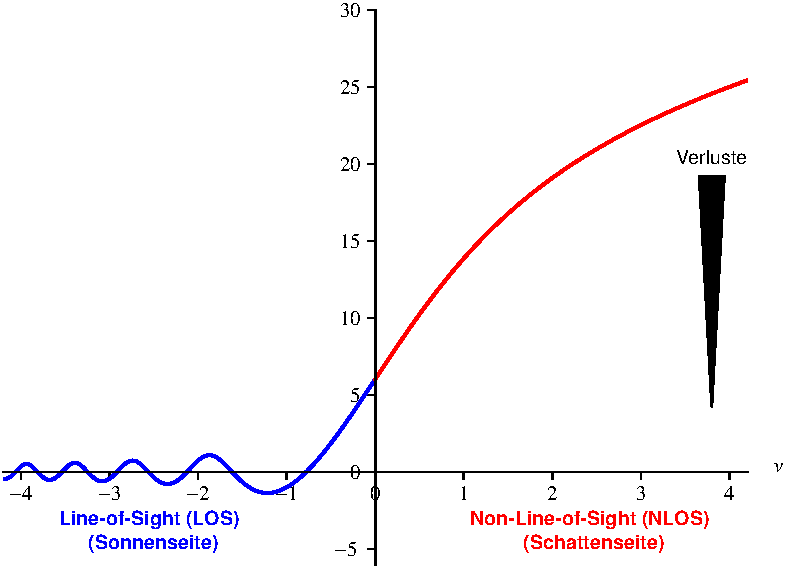
\includegraphics[width=\textwidth]{papers/fresnel/pgf/beugungsverluste.pdf}
    \caption{
        Diagramm der Beugungsverluste $L_{\unit{\decibel}}$
        \label{fresnel:Fresnel-Diagram}
    }
\end{figure}

